\documentclass[12pt]{document}  % default square logo 
%\documentclass[12pt,beltcrest]{ociamthesis} % use old belt crest logo
%\documentclass[12pt,shieldcrest]{ociamthesis} % use older shield crest logo

%load any additional packages
\usepackage{amssymb}
% Korrektes Kodieren des in und outputs
\usepackage[T1]{fontenc}
\usepackage[utf8]{inputenc}
\usepackage{url}

\usepackage[backend=biber,style=numeric]{biblatex}
\addbibresource{refs.bib}

%Deutsche Silbentrennung
\RequirePackage{hyphsubst}%
\HyphSubstIfExists{ngerman-x-latest}{\HyphSubstLet{ngerman}{ngerman-x-latest}}{}


%input macros (i.e. write your own macros file called mymacros.tex 
%and uncomment the next line)
%\include{mymacros}

\title{Der Titel\\[1ex]     %your thesis title,
        kommt hier hin}   %note \\[1ex] is a line break in the title

\author{Max Mathys}             %your name
\college{Mathematisch-Naturwissenschaftliches Gymnasium Rämibühl}  %your college

%\renewcommand{\submittedtext}{change the default text here if needed}
\degree{Maturitätsarbeit}     %the degree
\degreedate{2016}         %the degree date

%end the preamble and start the document
\begin{document}

%this baselineskip gives sufficient line spacing for an examiner to easily
%markup the thesis with comments
\baselineskip=18pt plus1pt

%set the number of sectioning levels that get number and appear in the contents
\setcounter{secnumdepth}{3}
\setcounter{tocdepth}{3}


\maketitle                  % create a title page from the preamble info
\begin{abstract}
hji
\end{abstract}       % include the abstract


\begin{romanpages}          % start roman page numbering
\tableofcontents            % generate and include a table of contents
\listoffigures              % generate and include a list of figures
\end{romanpages}            % end roman page numbering

%now include the files of latex for each of the chapters etc
\chapter{Einleitung}
\begin{figure}[htb]
	\centering
		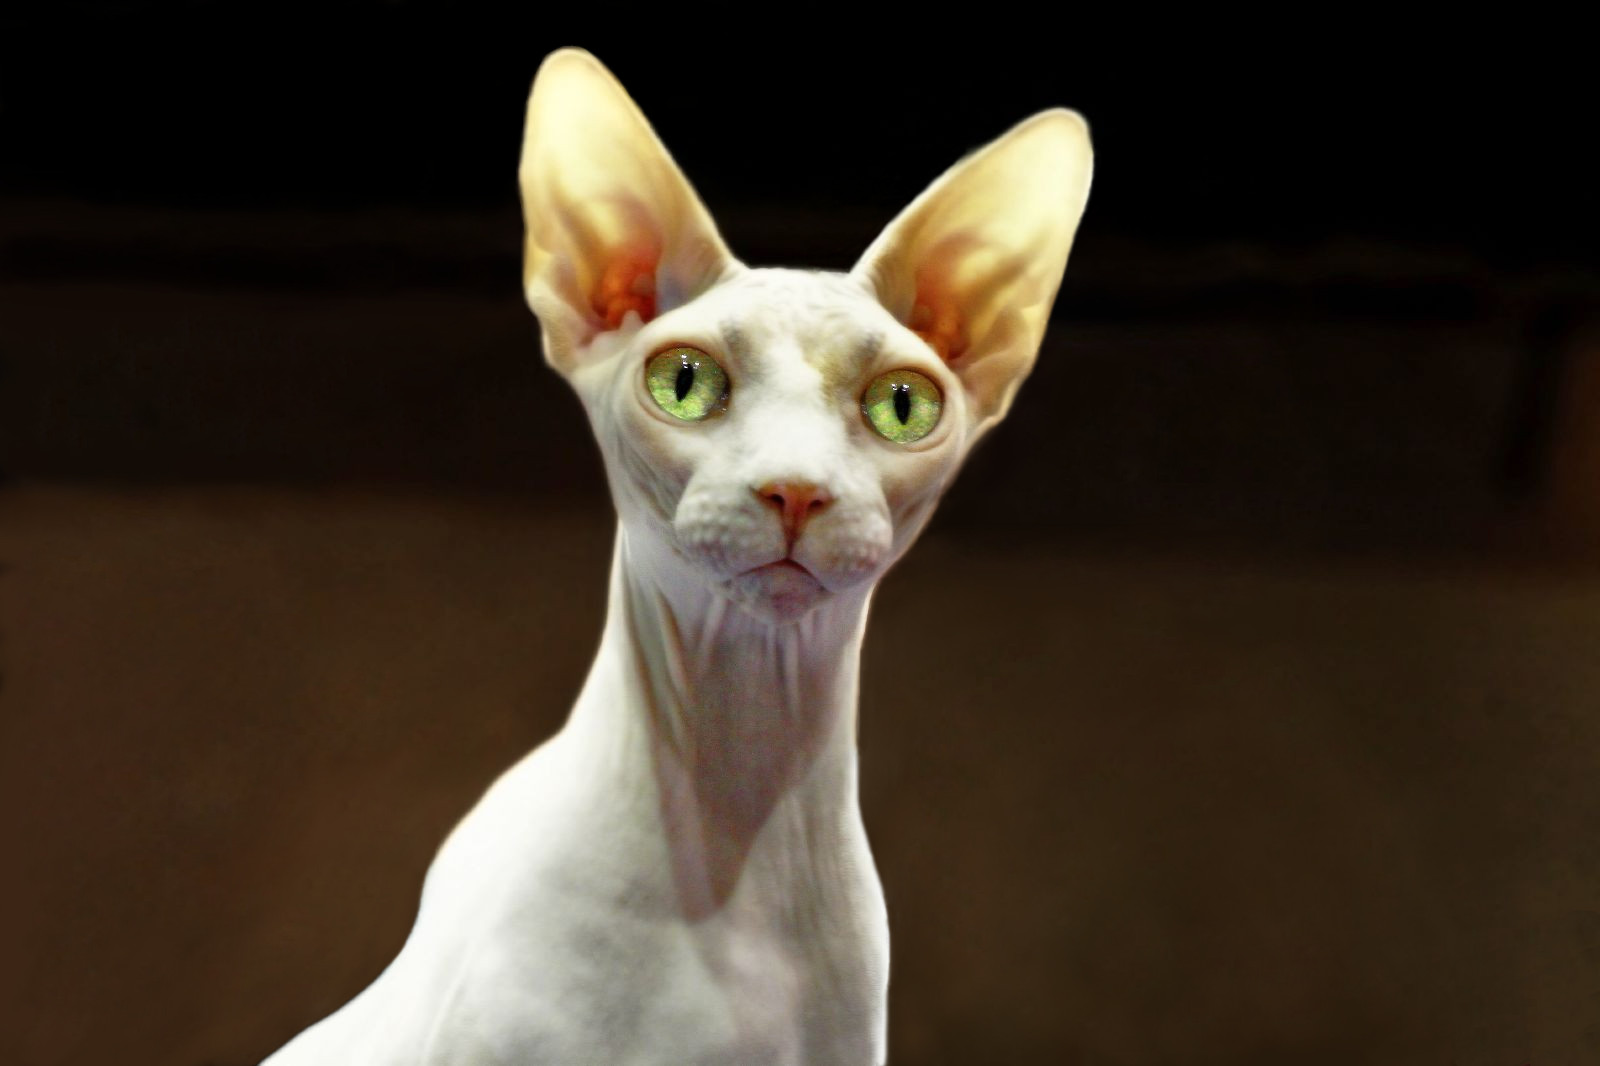
\includegraphics[width=0.7\textwidth]{images/cat.jpg}
	\caption{Eine Katze \cite{id}}
\end{figure}
ein text..

der ist gepastet. \cite{id}

\chapter{Grundlagen}

\section{2-Dimensionales Punktediagramm}
Das 2-Dimensionale Punktediagramm ist der am meisten verwendete Typ des Punktediagramms.

\subsection{Interpolation}
Für eine verbesserte Ansicht des Punktediagramms fügt man oft eine Linie ein, die alle im Punktediagramm vorhandenen Punkte verbindet. Sie stellt den Verlauf des Wertes zwischen den Datenpunkten dar.

Die unkomplizierteste, am meisten Verwendete Interpolation ist die \textbf{lineare Interpolation} (Abbildung \ref{fig:linear}). Zwei nebeneinanderliegende Punkte werden durch einer Gerade verbunden.

\begin{figure}[htbp]
	\centering
	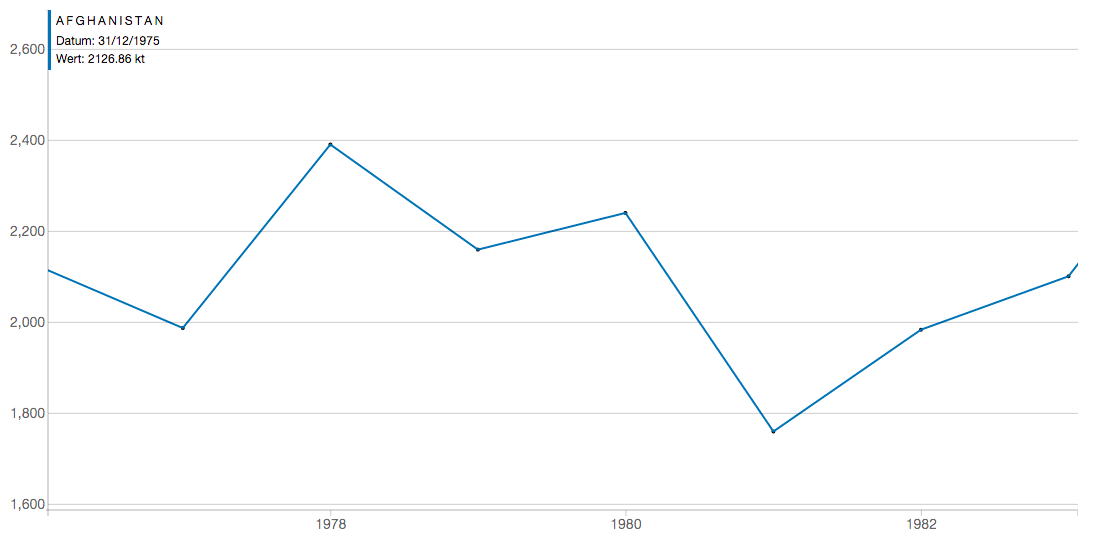
\includegraphics[width=0.80\linewidth]{images/linear}
	\caption[Lineare Interpolation]{Beispiel der linearen Interpolation am Datensatz des CO2-Verbrauchs von Afghanistan. <zu test layout verlinken>}
	\label{fig:linear}
\end{figure}

Die Interpolation mit Splines, der \textbf{Kubisch Hermitescher Spline} (Abbildung \ref{fig:cardinal}).

\begin{figure}[htbp]
	\centering
	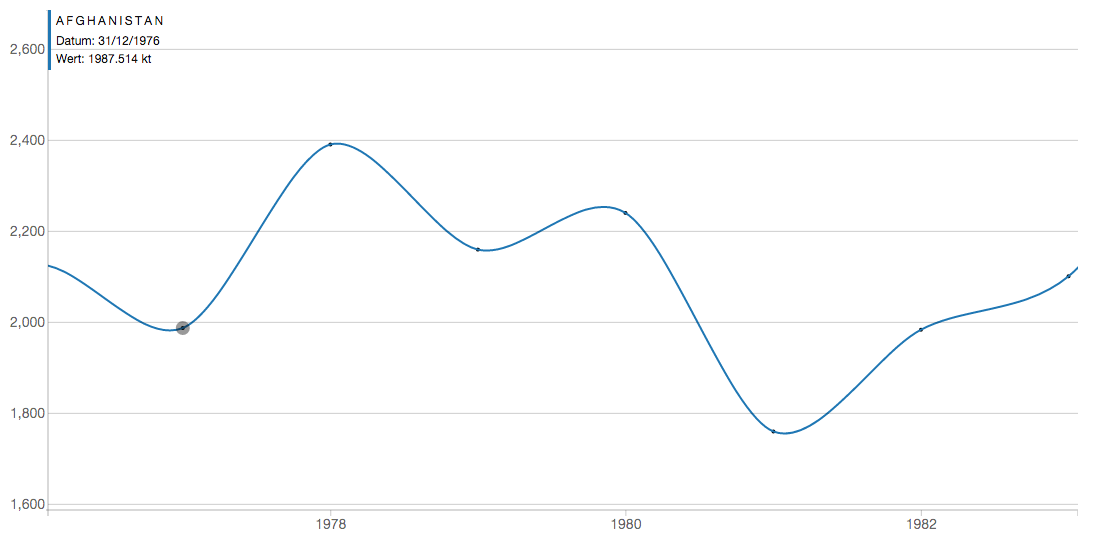
\includegraphics[width=0.80\linewidth]{images/cardinal}
	\caption[Kubischer Hermitescher Spline]{Beispiel des Kubischen Hermetischen Spline am Datensatz des CO2-Verbrauchs von Afghanistan <zu test layout verlinken>}
	\label{fig:cardinal}
\end{figure}

\subsection{Linien}
\subsection{Tooltip}
\subsection{Anzeige von mehreren Datensätzen}

\section{3-Dimensionaler Punktediagramm}

\subsection{Kamera}
\subsection{Projektion}
\subsection{Orthogonale und Perspektivische Projektion}
\subsection{Transition zwischen Projektionen}

\section{n-Dimensionaler Punktediagramm}
\chapter{Praktischer Teil\label{chapter:praktischer_teil}}

% visualisierungspipeline @ p 15
% ---> vier varianten; nur erste (bilder) und dritte (interaktiv), vierte (interaktiv, api, query, siehe yaho lol) variante üblich, vorteile/nachteile (loading time, browserunterstützung, speichern)
% beschreiben, welche variante man braucht.
% beschreiben was "Daten, F, M, R, Bild" in unserem Beispiel sind. f filtering m mapping r rendering
\chapter{Reflexion}


%now enable appendix numbering format and include any appendices
\appendix

%next line adds the Bibliography to the contents page
\addcontentsline{toc}{chapter}{Bibliography}
%uncomment next line to change bibliography name to references
\printbibliography

\end{document}

